\documentclass[]{article}

%%%%%%%%%% Packages/Macros %%%%%%%%%%
\usepackage{graphicx}
\usepackage{hyperref}
\usepackage{caption}
\usepackage{subcaption}
\usepackage{float}

%%%%%%%%%% Margins %%%%%%%%%%
\addtolength{\textwidth}{1.0in}
\addtolength{\textheight}{1.00in}
\addtolength{\evensidemargin}{-0.75in}
\addtolength{\oddsidemargin}{-0.75in}
\addtolength{\topmargin}{-.50in}

%%%%%%%%%% Graphics %%%%%%%%%%
\graphicspath{ {images/} }

%%%%%%%%%% Document %%%%%%%%%%
\begin{document}

\title{XSEDE Bibliometrics Proposal}
\author{
	Gregor von Laszewski \and
	Fugang Wang \and
	Timothy D. Whitson
}
\maketitle

\section{Compute Canada and XSEDE Comparison}

\begin{figure}[H]
    \centering
    \begin{subfigure}{.5\textwidth}
	    \centering
	    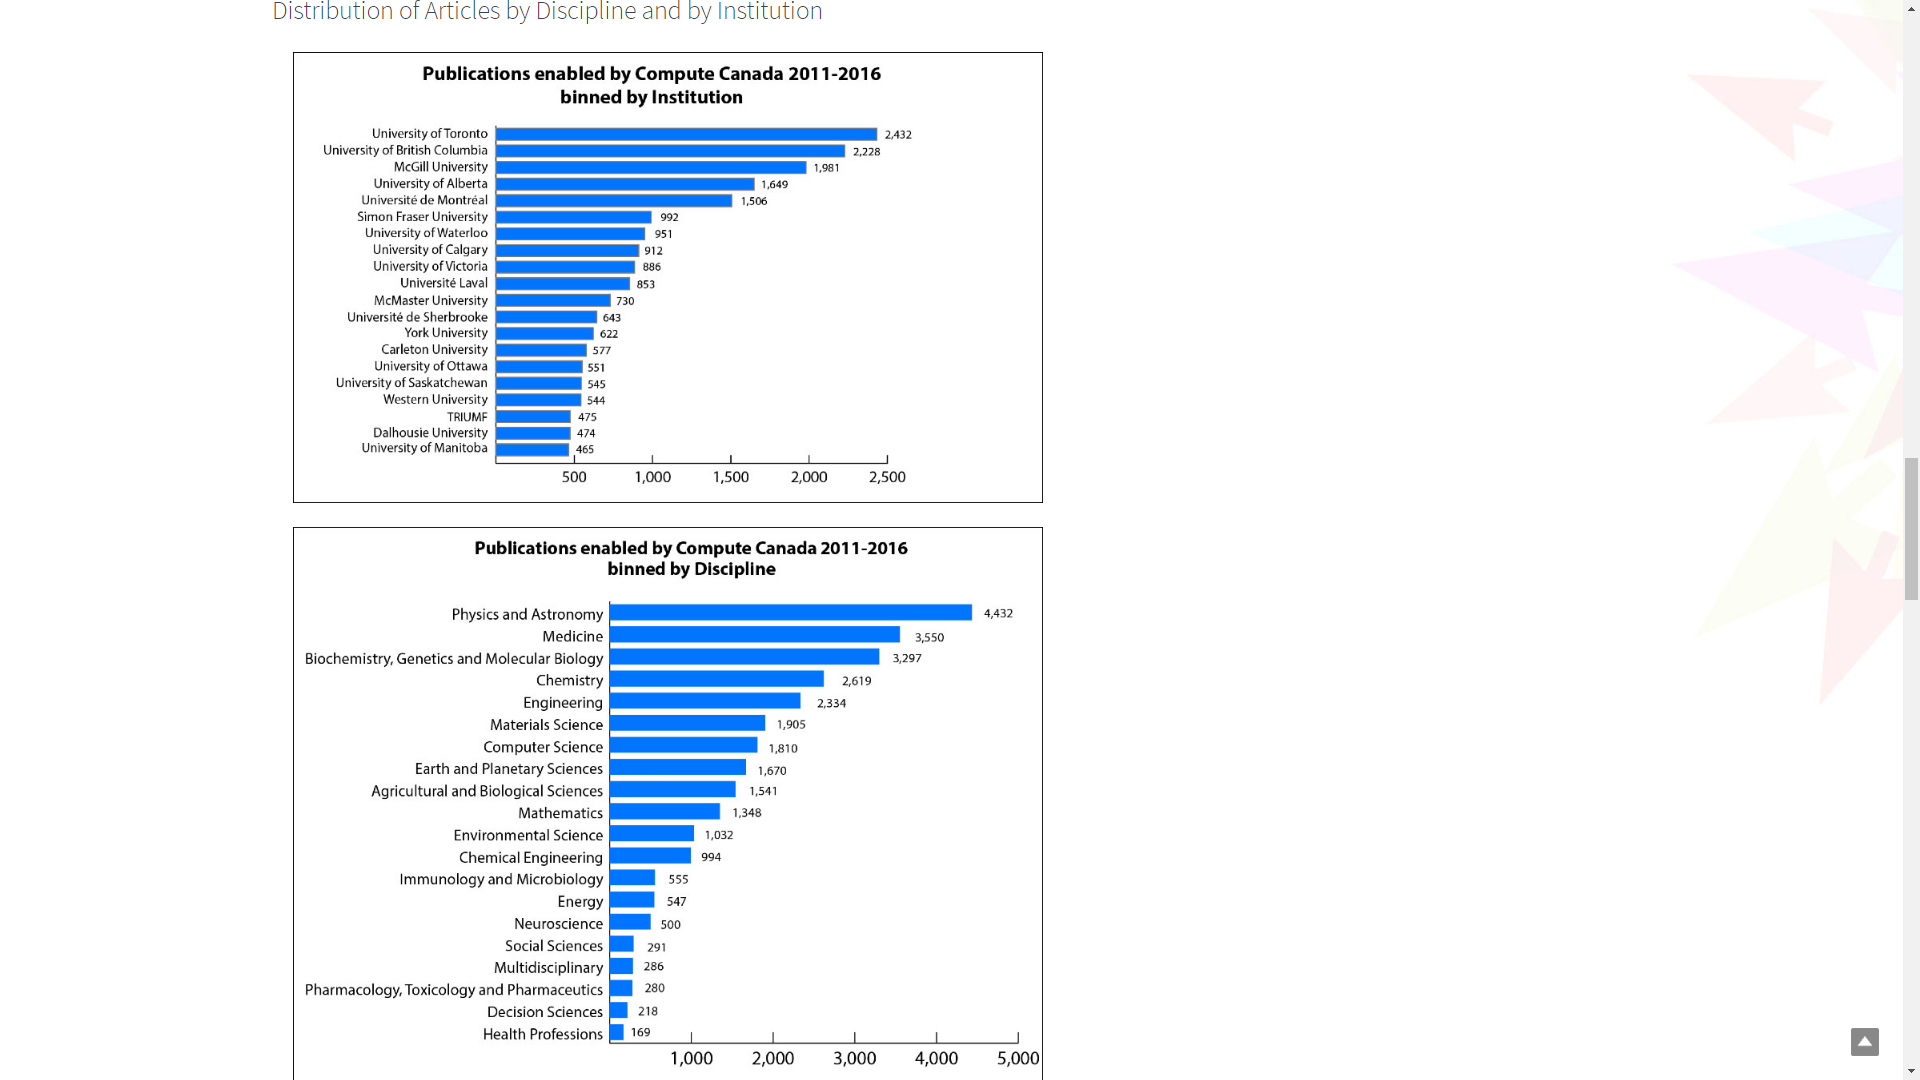
\includegraphics[width=.9\linewidth]{cc.png}
        \caption{Compute Canada Metrics}
        \label{Fig.1}
    \end{subfigure}%
    \begin{subfigure}{.5\textwidth}
	    \centering
	    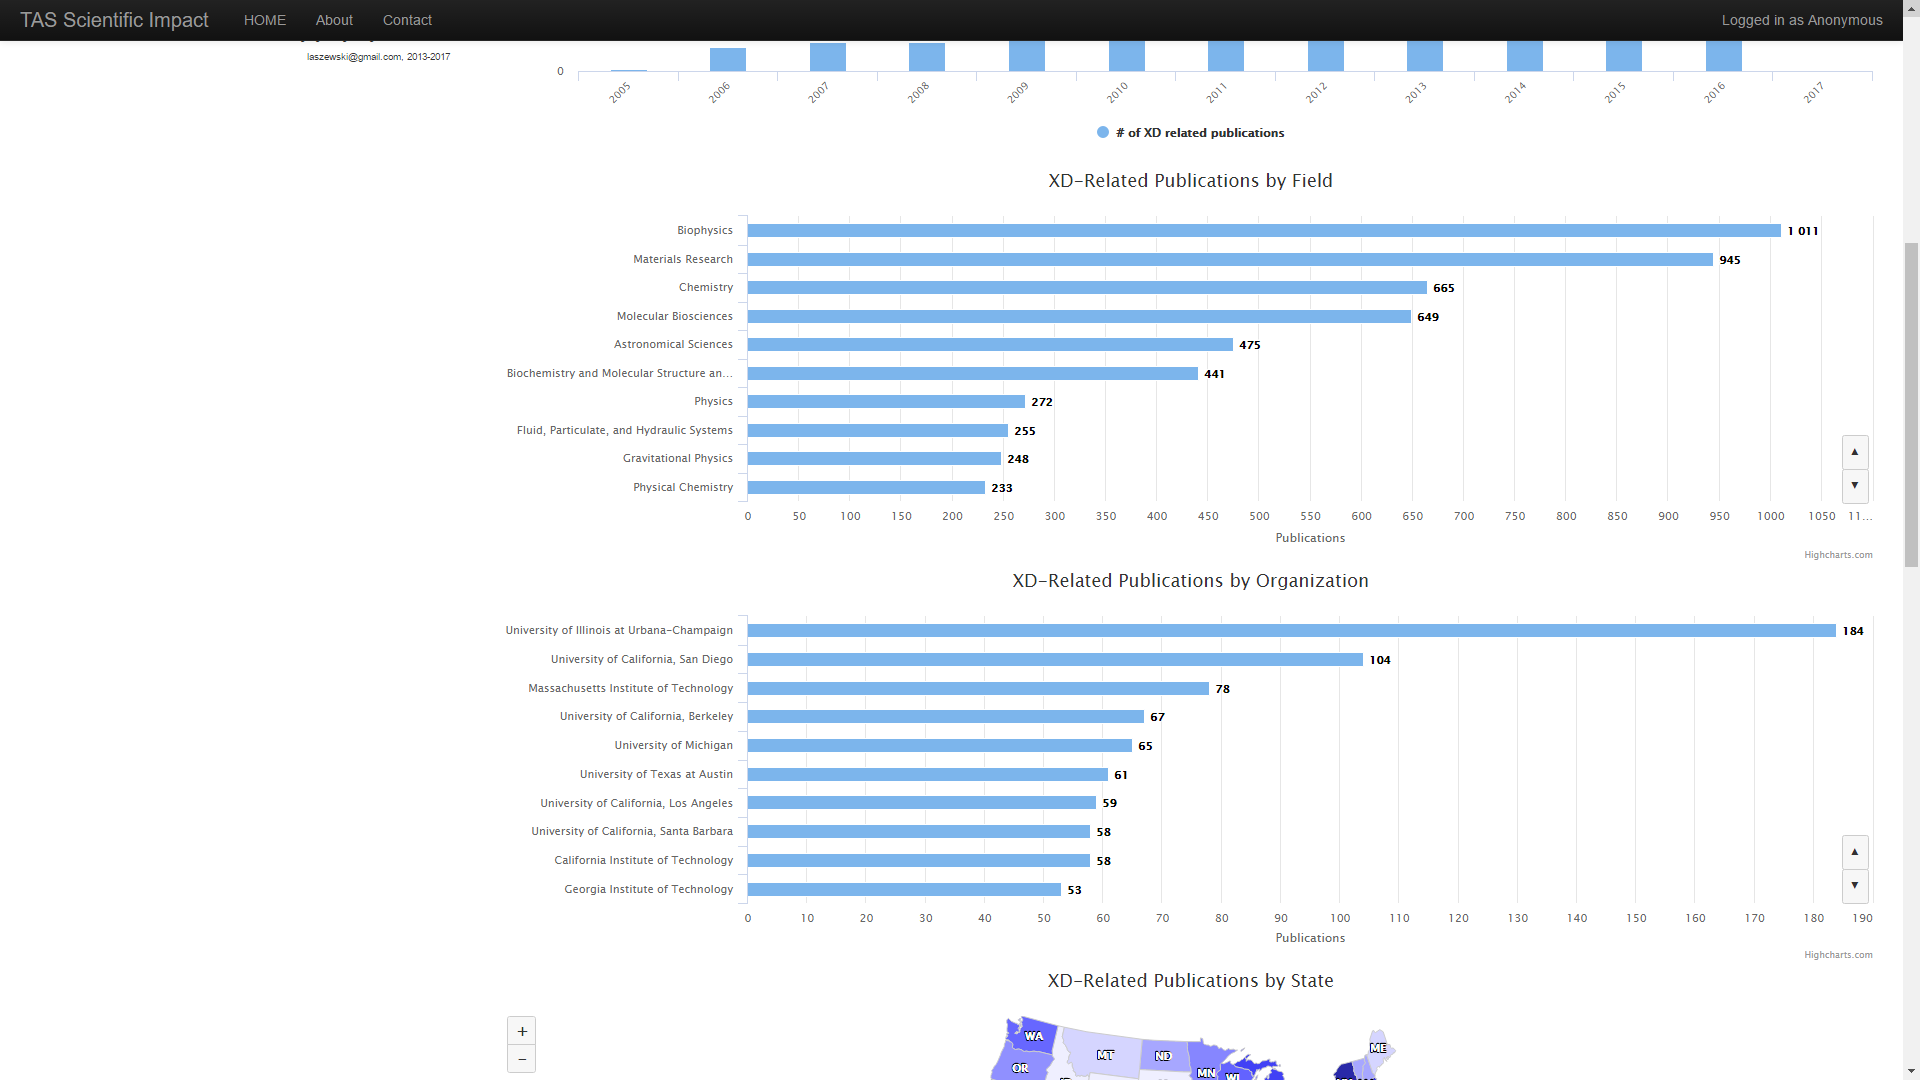
\includegraphics[width=.9\linewidth]{tas.png}
        \caption{Our Metrics}
        \label{Fig.2}
    \end{subfigure}
\end{figure}

Currently, we can produce similar charts to Compute Canada for institution and field metrics. However, Compute Canada has comparisons of their database with others to determine the impact of Compute Canada. To create a similar metric, we need access to publications outside of XSEDE. I will explore other sources for this data.

\section{Future Data Sources}

\subsection{NSF FastLane}
I could not find any information on gaining access to the NSF FastLane database. In particular, most of the documentation about FastLane describes the typical usage for academic institutions who use FastLane to secure funding. The registration process is outlined \href{https://www.fastlane.nsf.gov/a0/about/registration.htm}{here}.

\subsection{research.gov}
I had similar results using research.gov. They often reference the NSF programs, such as FastLane. They do have a portal that displays research spending by year (by institution), which could possibly be referenced \href{https://www.research.gov/research-portal/appmanager/base/desktop?_nfpb=true&_eventName=viewQuickSearchFormEvent_so_rsr}{here}.

\subsection{Elsevier Scopus}
Elsevier is a paid service and is used by Dr. Borner. Their Scopus service claims to be the largest bibliographics database in existence.\cite{borner}

\subsection{Thomson and Reuter Web of Science, InCites}
Thomson and Reuter have multiple databases for bibliometrics, inlcuding Web of Science and InCites. Drs. Ding and Borner have both used these in their research.\cite{borner}\cite{ding}

\subsection{Others to look into}
\begin{itemize}
\item SciELO
\item science.gov
\end{itemize}

\bibliography{proposal}
\bibliographystyle{acm}

\end{document}
